\section{Problemrapportering}
Projektet kommer att använda utvecklas agilt, med hjälp av scrum, för mer information om hur vi har anpassat scrum efter vår situation läs Appendix A i dokumentet projektplan som . Under dagliga scrum-standups där iterationens utveckling redogörs har varje person har en skyldighet att rapportera problem som uppstår och kan tänkas uppstå. Problem får sedan bearbetas och diskuteras om det är så att en enskild person inte kan lösa dem. Under gruppmöten kommer även större mer övergripande problem som rör flera medlemmar eller hela gruppen diskuteras. \\
Problem kommer därför att rapporteras på flera sätt, beroende på dess storlek och betydelse.
\subsection{Arbetsflöde}
För att kunna arbeta agilt behövs ett system för att spåra arbetet, där har gruppen valt att använda Trello\cite{website:trello} med anledningen att det är ett lättanvänt och väl beprövat verktyg.
\begin{figure}[h]
\begin{center}
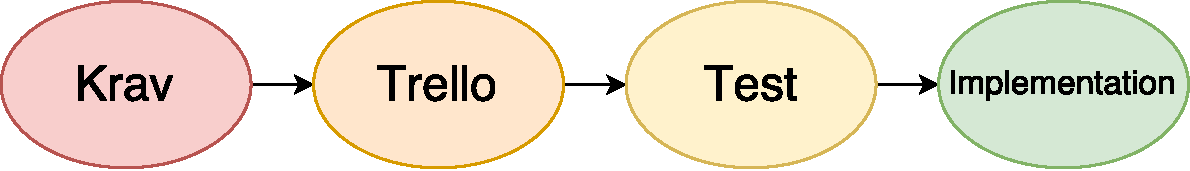
\includegraphics[scale=0.75]{tracability}
\caption{En illustration över arbetets spårbarhet.}
\label{fig:tracability}
\end{center}
\end{figure}
\\
För att uppnå spårbarhet och kunna leverera mot kundens krav har alla Trello-kort en etikett med id för det krav i kravspecifikationen som de implementerar och en beskrivning över de testfall som validerar dess funktionalitet. Se figur \ref{fig:tracability} för en illustration över processen.
I de fall som korten valideras med hjälp av automatiserade tester kommer en lista på testfall som förväntas passera förses, och i de fall manuella tester krävs kommer en detaljerad steg-för-steg-lista förses.
